\chapter*{修订文档说明}
为了逐步完善《全局光照技术》图书的内容,提高其准确性和严谨性,以及让广大读者及时获取最新的修订内容,特制作本《全局光照技术》修订文档。读者可以从以下地址获取本文档的最新版本:

\url{https://github.com/thegibook/revision}

出于易阅读性和修订内容的重要性考虑,本修订文档不包括错别字,多字,少字,同音字,笔误等文法错误,这种类型的错误通常不会影响知识或句子的理解,读者应该能够比较容易地识别这样的错误,因为这些内容加到本文档会大大增加篇幅。对于这种类型的修订,如果读者感觉拿不定判断,仍然可以在上述网站的issue页面进行搜索以对比相关修订内容。

为了便于阅读,本段后面的内容对应于一个修订的各个部分的示例,其中标题部分是对应的修订序号以及对应的起始页,页码是对修订进行索引的唯一方式,所有的修订会按照页码顺序进行排序。标题下面注明了修订内容错误的类型,反馈读者,以及对应的反馈页面。

\begin{revision}{p123}{理解错误}{sYeaLumin}{\url{https://github.com/thegibook/revision/issues/80}}	
\end{revision}

紧接着标题的,是图书修订后的正文内容,这部分内容会包含和原书修订后一模一样的排版,它以段为单位,例如如果是某个段内的两个句子发生了修改,这里就会列出修订后的图书中这两句所在的整个段落。

每个修订涉及的所有更改都会出现在这里,如果一个完整的小节内容被修订,那么这里就会列出该节全部的内容,同时包括对应的小节名称,以及其他所有的图片,公式等完全一样的排版。

\begin{myshaded}
	这部分会对修订的思路加以简要说明,这部分文字不会出现在修订后的图书正文内容中,它可能包含一些对原始内容错误原因的解释,引发的其他思考等内容。
\end{myshaded}




\chapter*{修订致谢}
一本好的图书,除了作者自己的所有创作过程,也离不开广大读者的反馈和建议,从某种程度上说,后者的力量和贡献更大,因为读者拥有更广泛的智慧和知识面。没有读者的支持和帮助,本书就不可能走向优秀,所以在这里诚挚感谢各位读者的反馈,相关的反馈报酬请参阅本书的反馈网站。

这里列出所有对本次修订有贡献的所有读者,当然有一些反馈例如错字是没有出现在本文档中的,但是这些读者的名字仍然会出现在下面,这里排名不分先后:

sYeaLumin, sYeaLumin , sYeaLumin 





\chapter*{修订内容}
\setcounter{revision}{0}


% -----------piv----------------
\begin{revision}{piv}{概念解释有误}{TYJia}{\url{https://github.com/thegibook/revision/issues/89}}
	有限元不是对无限空间的积分分解,而是对连续空间的积分分解(连续空间的离散化)
\end{revision}

\begin{itemize}
	\item \textbf{基于有限元分解的辐射度理论 } 有限元分解是一种常见的积分计算方法,它将一个沿连续空间的积分分解为一个有限纬度(称为一个有限元)的积分,在每个纬度,我们只需要求出该有限元的均值,并可以很容易地计算出光照积分方程。在辐射度理论中,通常我们通过Monte Carlo等方法预计算出每个有限元的均值,供渲染时渲染方程的实时计算。
\end{itemize}



% -----------p27----------------
\begin{revision}{p27}{公式有误}{topameng}{\url{https://github.com/thegibook/revision/issues/16}}
指数上的符号位错了,这里应该没有负号
\end{revision}
相反,给定$F(\mu)$,通过傅里叶反变换可以获得$f(t)$:

\begin{equation}
\renewcommand\theequation{1.21}
	f(t)={\rm \int}^{\infty}_{-\infty}F(\mu){\rm e}^{j2\pi\mu t}{\rm d}\mu
\end{equation}




% -----------p34----------------
\begin{revision}{p34}{图示错误,解释补充}{Qinja}{\url{https://github.com/thegibook/revision/issues/95}}
	首先±1/ΔT点比起图(c)应该往0点靠近,然后把两个线交叉表达出来,相加得到的值不一定是一条直线吧?这里看前几次都没看懂,看完了理论才知道啥意思。
\end{revision}

图\ref{f:intro-sampling-aliasing}显示了上述这种采样后函数的傅里叶变换图示,其中图\ref{f:intro-sampling-aliasing}(a)为原始连续带限函数$f(t)$的傅里叶变换,图\ref{f:intro-sampling-aliasing}(b)~(d)则表示采样后函数的傅里叶变换,如前所述,$1/\Delta T$是用于生成采样后函数的采样率。由此可以看出,为了保持对原始信号的重建能力,我们需要使用足够的采样率来保证$F(\mu)$的完整性,在图\ref{f:intro-sampling-aliasing}(c)中,采样率刚好能够保持$F(\mu)$,因此我们可以使用一个低通过滤器(如图中的虚线线段所示)来完全得多原始信号的所有频率信息,因此能够被完美重建,这部分的内容将在下一节讨论。而在图\ref{f:intro-sampling-aliasing}(d)中,采样率低于保持不同$F(\mu)$拷贝的最小采样率要求,因此它无法被完美重建。

\begin{figure}
\renewcommand\thefigure{1.33}
	\sidecaption
	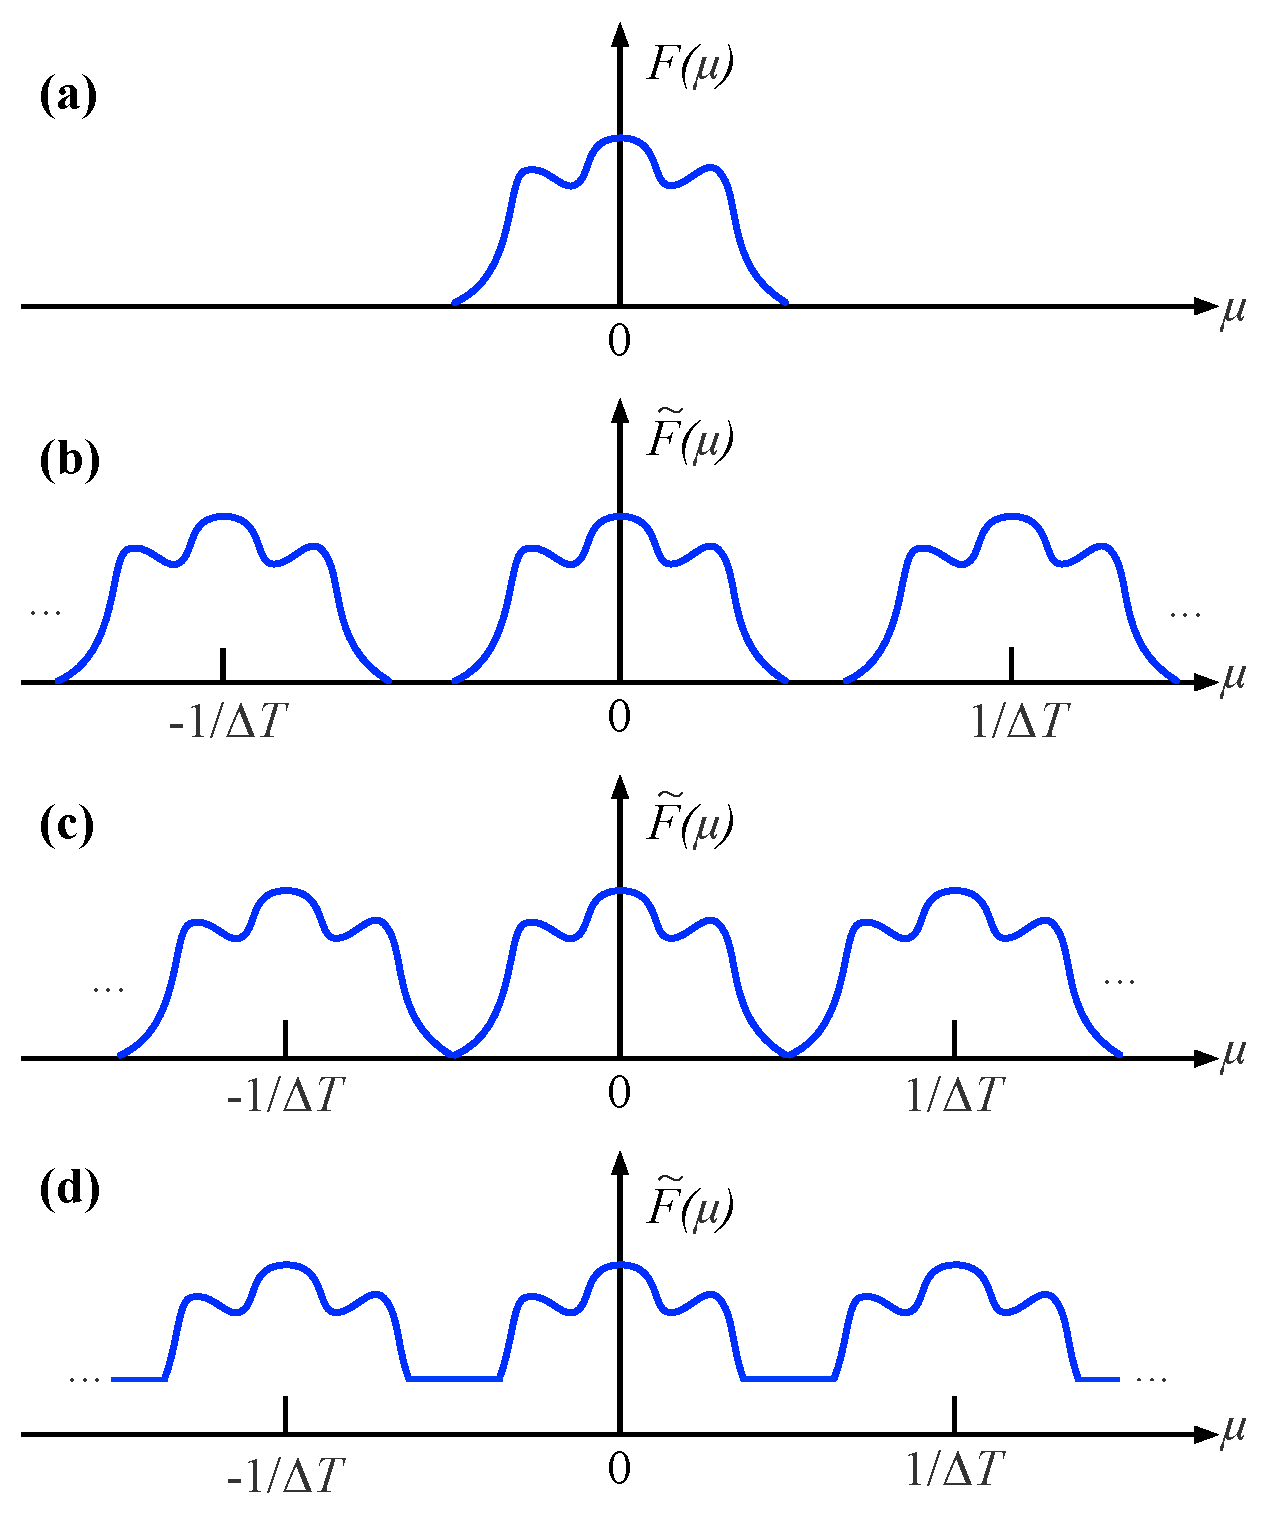
\includegraphics[width=0.65\textwidth]{figures/intro/sampling-aliasing}
	\caption{(a)为一个带限函数的傅里叶变换,(b)-(d)分别为过采样,临界采样和欠采样条件下采样后函数$\tilde{f}(t)$的傅里叶变换$\tilde{F}(\mu)$}
	\label{f:intro-sampling-aliasing}
\end{figure}

在图\ref{f:intro-sampling-aliasing}(d)中,由于采样后函数的周期变小,因此各个拷贝的相邻位置处发生重叠,如图\ref{f:intro-sampling-aliasing}(d)的红色线段部分所示,这部分的频率信息表现为相互叠加部分的和(这是因为式1.35是各个拷贝的和式),即这部分的频率信息被修改,因此发生了走样(aliasing)。实际上alias这个单词的意思是别名,这里的本意实际上是指某些频率信息被其他的频率值代替。可以想象,此时使用能够覆盖一个周期的低通过滤器,是不可能完全保留原始函数的所有频率信息的,因此无法被完美复原。

\begin{myshaded}
	这个反馈很好,d图确实应该靠近一点。这个反馈让我感觉交叉部分应该特别解释一下,一个是这个图来源的参考资料(网上大多数)大多都是线性的频率分布,因此交叉部分可能是一个直线,但是本书我们使用了一个不规则的频率分布,因此可以是一个任意形状,所以把交叉部分表达出来确实能更好地解释;另外一个是这个交叉的意义需要在书中特别解释一下。
\end{myshaded}



% -----------p63----------------
\begin{revision}{p63}{描述错误}{lonelyWaiting}{\url{https://github.com/thegibook/revision/issues/13}}
描述: 从[0,1]重映射到[0.5,1]
错误之处: 实际给出的公式是将其从[0,1]映射到[0.25,1]
\end{revision}
\noindent 对于Walter的近似方法,Disney将粗糙度参数$\alpha_g$从$[0,1]$ 重映射到$[0.25,1]$,即:$\alpha_g=(0.5+roughness/2)^2$,以使$G$函数随着粗糙度变化更平滑;对于Secondary lobe,则直接使用一个固定的粗糙度参数0.25。



% -----------p72----------------
\begin{revision}{p72}{公式错误}{Qinja}{\url{https://github.com/thegibook/revision/issues/101}}
	在GI书的P72页,第二行,公式1.73,对比有误。连续乘法的第4项$(1/\eta)^2$可以删去。其实不删去的话,一眼就看出来有问题了。第三项分子和第四项分母一样不能约分?
\end{revision}

\noindent 则Walter定义的BTDF可以写为:

\begin{equation}\renewcommand\thefigure{1.73}
	f_t(\mathbf{i},\mathbf{o},\mathbf{n})= \cfrac{|\mathbf{i}\cdot\mathbf{h}_t|}{|\mathbf{i}\cdot\mathbf{n}|}\cdot \cfrac{|\mathbf{o}\cdot\mathbf{h}_t|}{|\mathbf{o}\cdot\mathbf{n}|}\cdot \cfrac{\eta^2}{(\mathbf{i}\cdot\mathbf{h}_t+\eta(\mathbf{o}\cdot\mathbf{h}_t))^2}\cdot (1-R_F(\mathbf{i},\mathbf{h}_t))G(\mathbf{i},\mathbf{o},\mathbf{h}_t)D(\mathbf{h}_t)
\end{equation}





% -----------p88----------------
\begin{revision}{p88}{概念解释错误}{onamiforest}{\url{https://github.com/thegibook/revision/issues/61}}
IF的部分,第六行"并同时将程序计数器的地址增加32位(或者64位)"后面两个位字应该去掉,即 增加32(或者64)
\end{revision}

\setcounter{footnote}{1}
\begin{enumerate}
	\item \textbf{IF: } 获取指令(instruction fetch)阶段,处理器从一级指令缓存L1I\$获取一个32位\footnote{如果是64位机,则指令长度为64位。}的指令,该操作通常具有1个时钟周期的延迟。在这个阶段,一个称作程序计数器(program counter,PC)\myindex{程序计数器}{program counter}的寄存器用来保存当前被执行指令在缓存中的地址,它被用于提供给PC预测器(PC predictor),PC预测器用这个地址直接获取指令缓冲区的一个指令,并同时将程序计数器的地址增加4(或者8,因为每条指令的长度为4个字节),以将程序计数器更新到下一个连续程序计数器。这种简单的预测方式通常会在当前指令处发生分支或跳转的时候出现错误,从而导致下一次指令获取出现指令缓存失效,我们上一节讲述的指令预取技术将在这个阶段进行计算。
\end{enumerate}

\begin{myshaded}
	这个反馈很好,这里地址增量是一个整数,所以并没有单位(实际上增量操作符所对应的具体位数是跟操作符本身有关的);但是这里程序计数器通常是按字节操作的,所以这里增量应该是4个字节(对应于32位)。
\end{myshaded}





% -----------p93----------------
\begin{revision}{p93}{解释补充}{Qinja}{\url{https://github.com/thegibook/revision/issues/104}}
	举例fsel操作符时,数字表意不明,代码中用到的是整数,到了这里就是小数,CPU不是会尽量用整数吗?为何一个是1.0没有f,一个是2.0有f?
\end{revision}
条件转移类似于C++中的三元操作符,在处理器中,一个浮点数条件转移操作符称作fsel,它是浮点数选择(floating-point selection)的简称,它具有如下的指令形式:

\begin{lstlisting}[language=C++]
fsel f0, f1, f2, f3 // f0 = ( f1 >= 0 ? f2 : f3 )
\end{lstlisting}

该指令直接将f1与0.0进行比较,然后直接选择f2或者f3,这是一个单条指令,不包含分支或者跳转。编译器往往能够将三元操作符直接转换为fsel操作符:

\begin{lstlisting}[language=C++]
	return a >= 0 ? b : c;	-->   fsel fr0,fr1,fr2,fr3
\end{lstlisting}

甚至如:

\begin{lstlisting}[language=C++]
// float a, b, c, d, e, f;
return ( a >= 0 ? b + 1 : c + 2 ) + ( d >= 0 ? e + 1 : f + 2 ) ;
\end{lstlisting}
也可以转换为:

\begin{lstlisting}[language=C++]
fr1 = a, fr2 = b, fr3 = c,
fr4 = d, fr5 = e, fr6 = f
fr0 = 1.0f, fr13 = 2.0f
fadds   fr12,fr2,fr0      ; fr12 = b + 1
fadds   fr11,fr3,fr13     ; fr11 = c + 2
fadds   fr10,fr5,fr0      ; fr10 = e + 1
fadds   fr9,fr6,fr13      ; fr9  = f + 2
fsel    fr8,fr1,fr12,fr11 ; fr8  = a >= 0 ? fr12 : fr11
fsel    fr7,fr4,fr10,fr9  ; fr7  = d >= 0 ? fr10 : fr9
fadds   fr1,fr8,fr7     ; return = fr8 + fr7
\end{lstlisting}

通过上面的示例可以看出,fsel对两个输入值都需要进行计算,即相当于计算了原来if条件语句的两个分支语句。然而即便如此,fsel带来的性能提升仍然十分明显,这得益于它直接省略掉了分支选择,尤其是当程序中有大量if条件语句并列,或者在一个循环语句中穿插if条件语句等情形,这些带来的处理器资源浪费极大。当然fsel只处理浮点数的比较,读者可以从\cite{a:ThePowerPCCompilerWritersGuide}了解更多信息。在\cite{a:DoggedDetermination:TechnologyandProcessatNaughtyDogInc.}中,Jason Gregory建议对于高性能部分,尽量使用fsel指令,并且拆分循环内的条件语句,尽可能地使用简单的,少分支的算法。

\begin{myshaded}
	这个反馈很好!我再仔细阅读了内容,发现关于fsel操作符讲的不够详细,导致了一些疑惑。fsel操作符是floating-point section的简称,所以它只处理浮点数的比较,所以1.0漏了f,关于fr之类的只是寄存器名称,并没有特别含义。fsel的意义其实就是因为浮点数的比较太耗时,会占用更多的时钟周期,所以导致指令管线产生更多气泡,fsel就是简化了浮点数的比较,它特别地只与0.0进行比较,这个比较会比单纯两个浮点数的比较快得多,这就是它能提升性能的原因
\end{myshaded}




% -----------p210----------------
\begin{revision}{p210}{计算错误}{	sYeaLumin}{\url{https://github.com/thegibook/revision/issues/73}}
	按位解码的代码举例与文字表述不符
\end{revision}
其次,他们充分使用GCN架构内置的的位解码方法来充分压缩每个参数的长度,使得图4.23中每个G-buffer中每个像素仅占用16位的存储空间。传统的着色器编程语言通常使用固定的包含1到4个分量内部图像格式,某些参数在实际中可能占用比一个分量更少的位置,这就会导致一定的浪费。GCN架构提供的解码方法\cite{a:Low-levelShaderOptimizationforNext-GenandDX11}可以对任何整数按位进行解码,这使得我们可以在帧缓存中存储任何长度(甚至超过4个分量)的数据,并且这个操作可以在1个GPU时钟周期内完成,例如以下代码分别取s变量二进制表示的$12\sim 16$、$6 \sim 11$和$1\sim 5$位,它们分别是5位、6位和5位的颜色分量:

\begin{lstlisting}[language=C++]
int r = s & 0x1F; 			  // 1 cycle
int g = (s >> 5) & 0x3F;	// 1 cycle
int b = (s >> 11) & 0x1F;	// 1 cycle
\end{lstlisting}



% -----------p211----------------
\begin{revision}{p211}{理解问题}{	sYeaLumin}{\url{https://github.com/thegibook/revision/issues/74}}
	表意不清:材质类型 or 材质类型组合?
\end{revision}

神秘海域4中的延迟着色阶段是使用计算着色器以块为单位进行渲染的,其中每个块包含$16\times 16$个像素点。在延迟着色阶段,计算着色器分两步处理块中像素的着色计算:
\begin{enumerate}
	\item 对每个块执行材质类型定义(material classification),以得到一个材质类型组合。
	\item 对每个材质类型组合分别执行一次计算着色器。
\end{enumerate}



% -----------p244----------------
\begin{revision}{p244}{名称术语}{	Liaoer}{\url{https://github.com/thegibook/revision/issues/83}}
	采样和抽样的疑惑
\end{revision}

全书对于sampling统一使用术语采样,不再有抽样和采样的区分。




% -----------p264----------------
\begin{revision}{p264}{公式有误}{jacktheLad}{\url{https://github.com/thegibook/revision/issues/35}}
	公式有误
\end{revision}
\paragraph{平稳分布}
设马尔可夫链在一个状态空间中从某个初始状态出发经历一定的时间后,各个状态$j$的离散分布概率为$\pi_{j}$,如果对任意状态$j$存在概率密度函数$\pi_j>0$,并使得:

\begin{equation}\renewcommand\thefigure{5.36}
	\sum^{n}_{i=1}\pi_i p_{ij}=\pi_j
\end{equation}

\noindent 即从所有其他状态转移到$j$状态的转移概率之和为状态$j$的概率分布,记为:

\begin{equation}\renewcommand\thefigure{5.37}
	\mathbf{\pi} \mathbf{P}=\mathbf{\pi}
\end{equation}



% -----------p310----------------
\begin{revision}{p310}{概念解释有误}{jacktheLad}{\url{https://github.com/thegibook/revision/issues/49}}
	过滤不仅指的是移除过高的频率,移除任何我们不想要的频率都可以称为过滤,所以才有高通滤波,低通滤波等等之分。
\end{revision}
\setcounter{footnote}{6}
这样就使得采样结果更平滑\footnote{过滤的本质实际上是移除部分频率,例如移除高频的低通过滤,或者移除低频的高通过滤。}



% -----------p840----------------
\begin{revision}{p840}{概念解释有误}{syaoming}{\url{https://github.com/thegibook/revision/issues/11}}
	第一段第四行,”提升数据读取和纹理缓存效率” 表述有误,Crassin 原文表述的意思是 ”提升数据访问合并和纹理缓存效率“,这里"数据访问合并"(data access coalescing)是 GPU 计算中的概念,文中的翻译忽略了关键的 coalescing 。
\end{revision}
对于节点内存池,所有的节点都存储在一个线性的全局内存中,例如可能 是全局纹理内存或常量内存,这方面可以参见本书前面第2章的内容。为了提供 更好的缓存行为,节点内存中的每个连续的内存块实际上由具有共同父节点的 $N\times N\times N$ 个(这里 $N = 2$)子节点组成,而不是像传统方法一样将每个节 点独立存储,我们称这些 $2\times 2\times 2$ 个节点组成一个节点片(node tile),如 图12.26左图所示。此外,为了使后面会讨论的遍历算法更加高效,节点数据中 的每一部分,即图12.25中的节点描述和体素数据被分别存储在一个独立的数组 中,这种结构也称为数组结构(structure of arrays,SOA),这是因为实际上在渲染算法中这两部分通常不会交叉,这样的结构能够提升数据访问合并(data access coalescing)和纹理缓存效率。













